\section{DEAP: IMPLEMENTAÇÃO DOS AGENTES}\label{sec:3deap-implagentes}

No capítulo anterior, foi abordada a utilização da biblioteca Gym para simular a interação de um sistema com um agente. Neste capítulo, o objetivo é verificar as funcionalidades providas pela biblioteca DEAP e como essas ferramentas foram utilizadas para representar indivíduos de uma população.

DEAP é uma biblioteca em \textit{Python} que promove a criação de protótipos e ideias na área da
computação evolutiva, com mecanismos que permitem a paralelização de tarefas. Suas áreas de aplicação, além da
programação genética, incluem: algoritmos genéticos, estratégias evolucionárias e otimização por enxame de partículas~\cite{deapdocs}.

Como dito, este trabalho, é voltado para a sua aplicação em PG.\@
O objetivo é implementar uma população de indivíduos,
representados como árvores ou listas de tamanho variável, que
representarão leis de controle para um sistema dinâmico.

Este capítulo descreve a implementação da população e dos indivíduos que a compõem, utilizando as ferramentas proporcionadas pela biblioteca. São analisados os parâmetros essenciais para a representação da solução, isto é, o tamanho da população, o número máximo de níveis das árvores, entre outros aspectos. Em seguida, é implementada a avaliação e seleção de indivíduos. Por fim, são definidos os operadores genéticos e o critério de término.

Já que a biblioteca DEAP será abordada ao longo deste capítulo, é proveitoso ter uma
visão geral das funcionalidades de cada módulo da biblioteca, explicitados na Figura~\ref{fig:3deap-modulos}.

\begin{figure}[H]
	\centering
	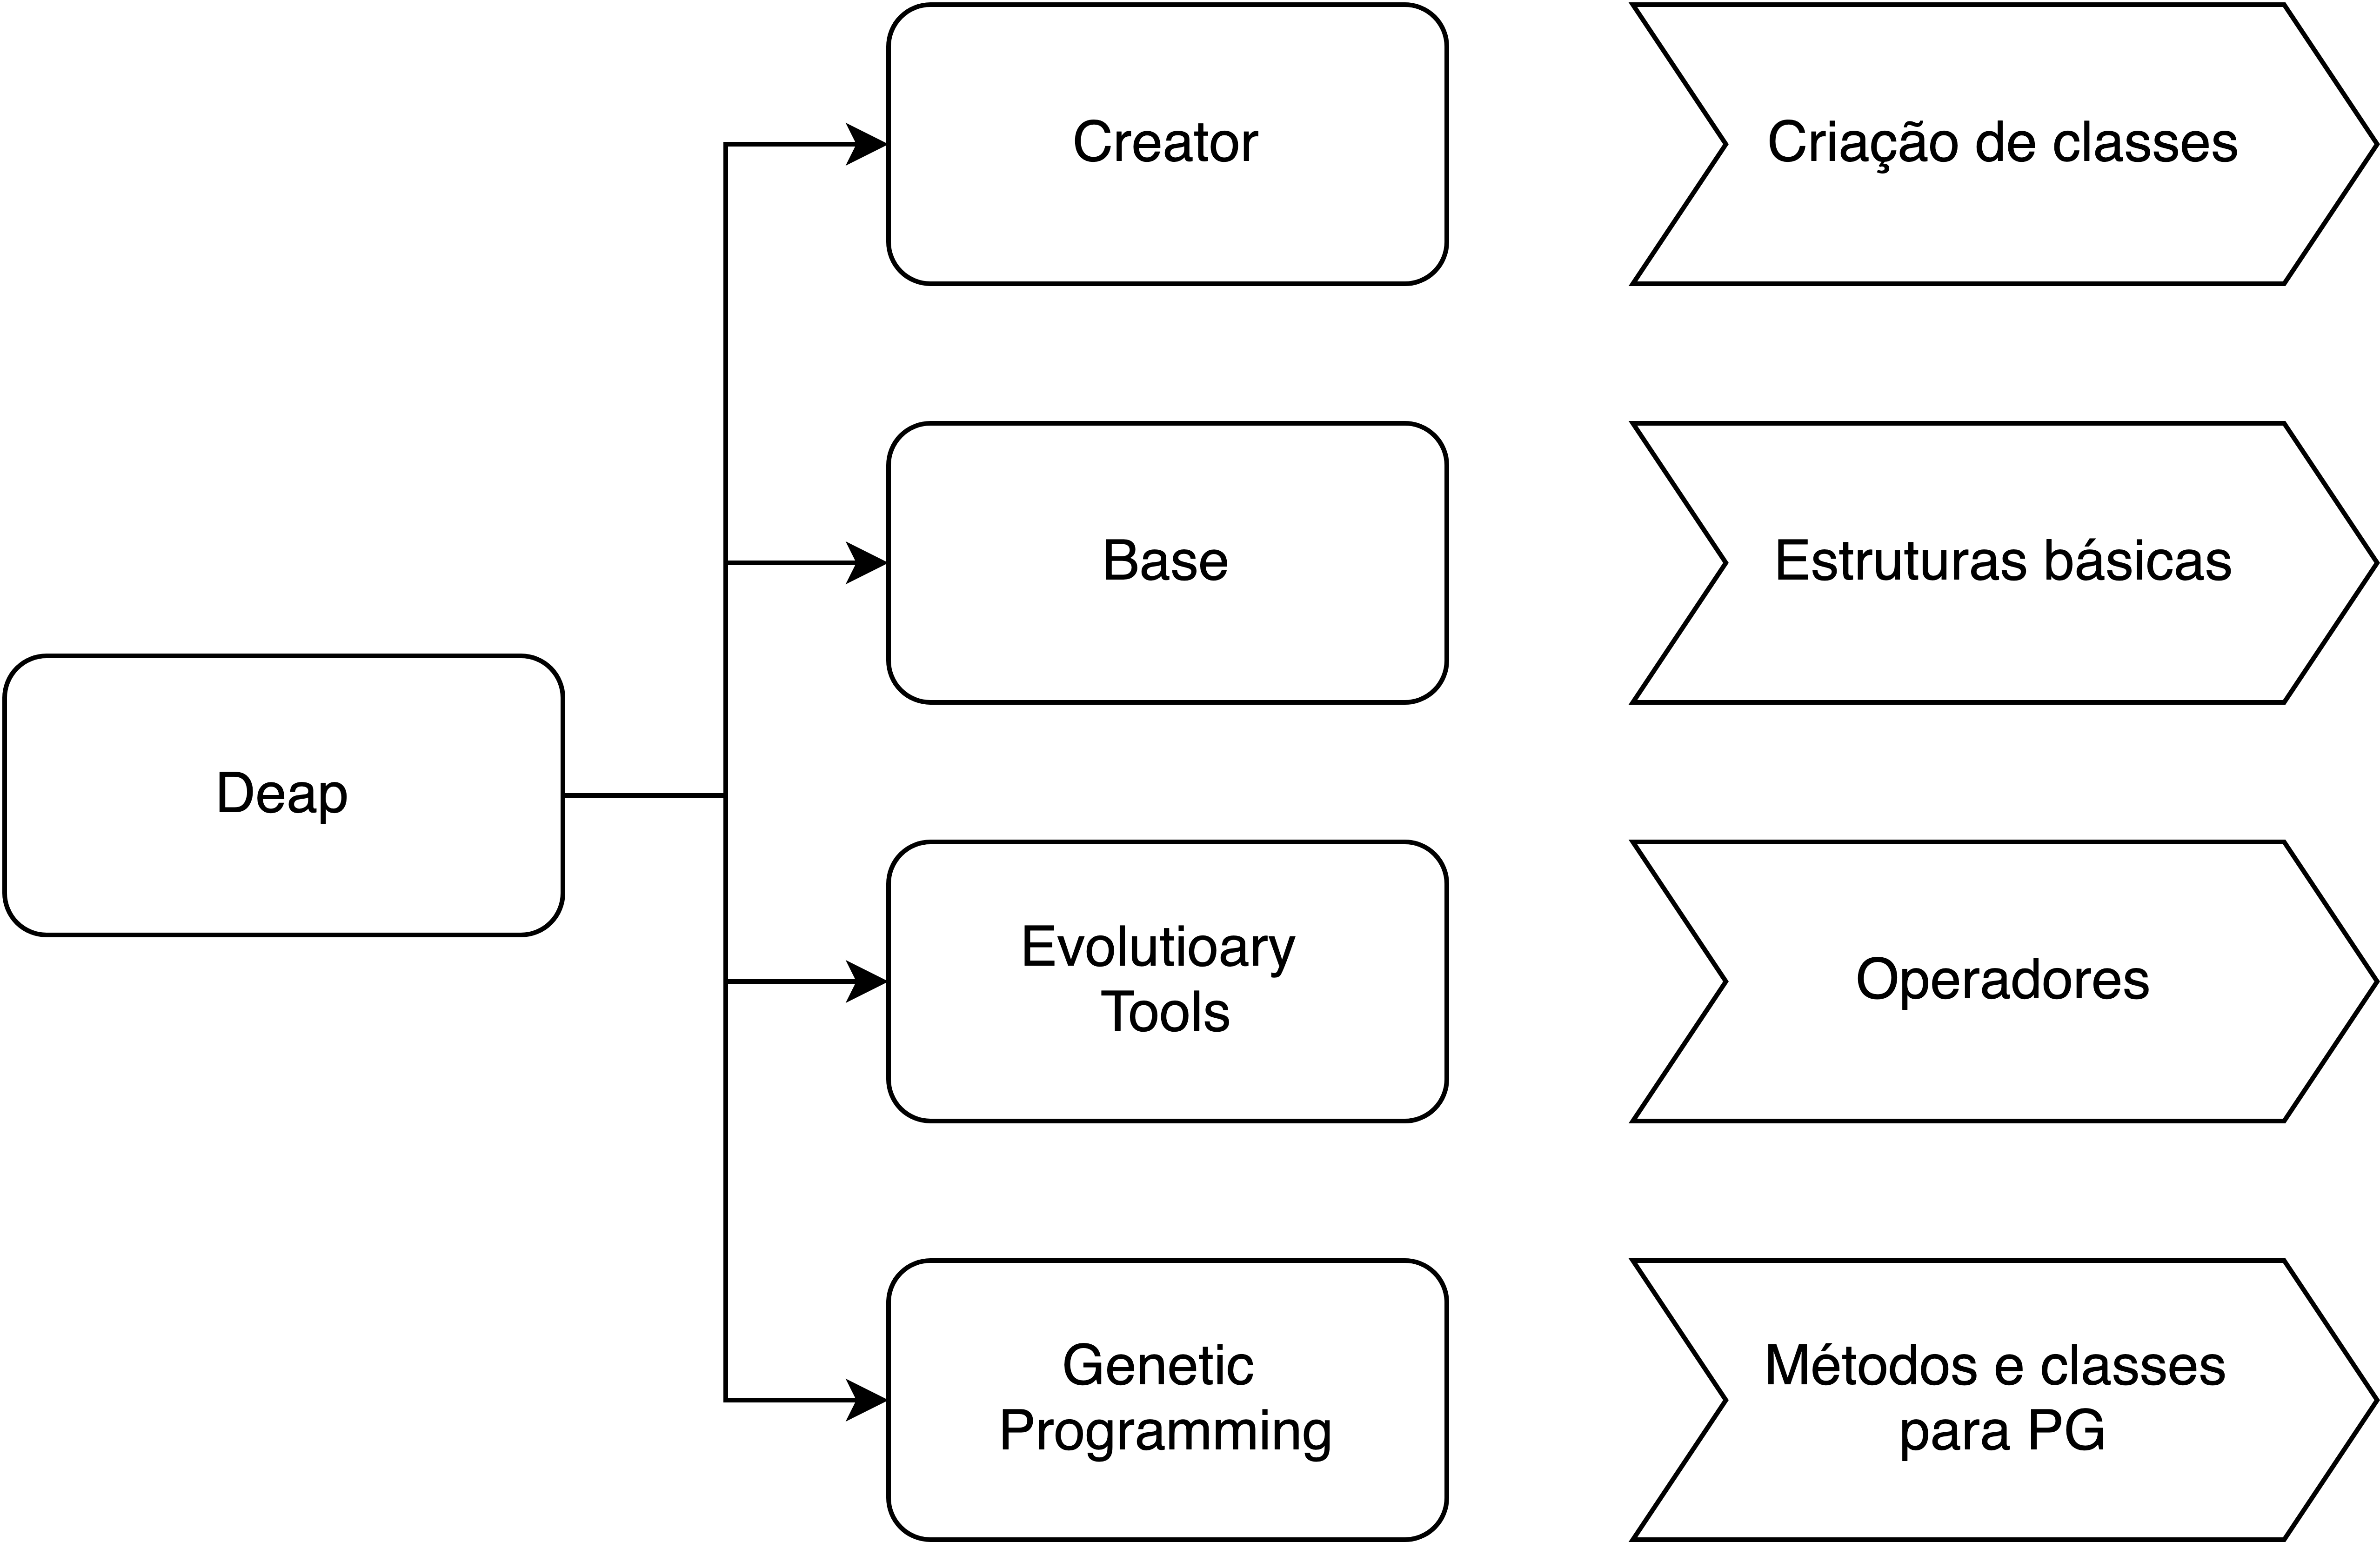
\includegraphics[width=0.7\linewidth]{02_desenvolvimento/03_Deap_Fig_Modulos.png}
	\caption{Módulos da biblioteca DEAP e suas funcionalidades.}\label{fig:3deap-modulos}
\end{figure}

\subsection{REPRESENTAÇÃO E INICIALIZAÇÃO}\label{ssec:3deap-represinic}

No Capítulo \ref{sec:1pg-apg}, a lista dos principais parâmetros que definem uma
implementação de PG é fornecida.\@ Neste capítulo, foi realizado um estudo dos aspectos referentes à representação de cada indivíduo e sua respectiva inicialização, tornando possível a criação de uma população inicial aleatória pronta para sofrer transformações ao longo do ciclo evolutivo.

\subsubsection{Representação}\label{sssec:3deap-representacao}

Para representar um indivíduo na PG deve-se definir: o conjunto de operações e o conjunto de variáveis terminais, denominados por $\mathcal{O}$ e $\mathcal{V}$, respectivamente. Geralmente essas duas entidades são agregadas em único conjunto denominado \textit{primitivo}. Logo, pode-se definir como \textit{conjunto primitivo} $\mathcal{P}$ o grupo que contém todas as funções (de diferentes aridades) e variáveis terminais que compõem os indivíduos da população.

As variáveis terminais podem ser \underline{constantes} ou \underline{entradas} vindas do sistema. As entradas são informações sobre as variáveis de estado do sistema. Geralmente, as constates são valores aleatórios, dentro de uma faixa, gerados na inicialização dos indivíduos. A existência de constantes aleatórias permite uma exploração maior do espaço de buscas, uma vez que as operações que atuam sobre esses números podem moldar coeficientes de uma lei de controle ótima para o problema.

Para o estudo de caso básico (pêndulo invertido), as variáveis terminais utilizadas estão descritas na Tabela \ref{tab:3deap-varterm}.

\begin{table}[H]
	\centering
	\begin{tabular}{l|l|l} \toprule
		{Variável Terminal} & {Significado} & {Tipo}\\ \midrule
		{$s$} & {Posição do carro} & {Entrada}\\
		{$\dot{s}$} & {Velocidade do carro} & {Entrada}\\
		{$\theta$} & {Ângulo do bastão} & {Entrada}\\
		{$\dot{\theta}$} & {Velocidade angular do bastão} & {Entrada}\\
		{$R$} & {Número gerado aleatoriamente ($-1,0<R<1,0$)} & {Constante}
		\\ \bottomrule
	\end{tabular}
	\caption{Variáveis terminais.}\label{tab:3deap-varterm}
\end{table}

Os operadores utilizados estão descritos na Tabela \ref{tab:3deap-operadores}, e foram escolhidos com base na literatura abordada (\cite{duriez17bookMlc}, \cite{koza92bookGp} e \cite{poli08GpFieldGuide}).

\begin{table}[H]
	\centering
	\begin{tabular}{l|l|l|l} \toprule
		\addlinespace[0.4ex] {Operador} & {Símbolo} & {Resultado} & {Aridade}\\ \midrule
		\addlinespace[0.4ex] {Soma} & {$+$} & {$a+b$} & {2} \\
		\addlinespace[0.4ex] {Subtração} & {$-$} & {$a-b$} & {2} \\
		\addlinespace[0.4ex] {Multiplicação} & {$\times$} & {$a\cdot b$} & {2} \\
		\addlinespace[0.4ex] {Divisão} & {$\div$} & {$a/b$} & {2} \\
		\addlinespace[0.4ex] {Raiz Quadrada} & {$\sqrt{}$} & {$\sqrt a$} & {1} \\
		%\addlinespace[0.4ex] {Raiz Cúbica} & {$\sqrt[3]{}$} & {$\sqrt[3] a$} & {1} \\
		\addlinespace[0.4ex] {Seno} & {$\sin$} & {$\cos{(a)}$} & {1} \\
		\addlinespace[0.4ex] {Comparação} & {$>$} & {\makecell{$a$, se $a\ge b$\\$b$, se $a<b$}} & {2} \\
		\addlinespace[0.4ex] {Sinal} & {sgn} & {\makecell{$1$, se $a\ge 0$\\$-1$, se $a<0$}} & {1}
		\\ \bottomrule
	\end{tabular}
	\caption{Conjunto de operadores lógicos e matemáticos.}\label{tab:3deap-operadores}
\end{table}

\begin{table}[H]
	\centering
	\begin{tabular}{l|l|l|l} \toprule
		{Operador} & {Símbolo} & {Resultado} & {Aridade}\\ \midrule
		{Soma} & {$+$} & {$a+b$} & {2} \\
		{Subtração} & {$-$} & {$a-b$} & {2} \\
		{Multiplicação} & {$\times$} & {$a\cdot b$} & {2} \\
		{Divisão} & {$\div$} & {$a/b$} & {2} \\
		{Raiz Quadrada} & {$\sqrt{}$} & {$\sqrt a$} & {1} \\
		%\addlinespace[0.4ex] {Raiz Cúbica} & {$\sqrt[3]{}$} & {$\sqrt[3] a$} & {1} \\
		{Seno} & {$\sin$} & {$\cos{(a)}$} & {1} \\
		{Comparação} & {$>$} & {\makecell{$a$, se $a\ge b$\\$b$, se $a<b$}} & {2} \\
		{Sinal} & {sgn} & {\makecell{$1$, se $a\ge 0$\\$-1$, se $a<0$}} & {1}
		\\ \bottomrule
	\end{tabular}
	\caption{Conjunto de operadores lógicos e matemáticos.}\label{tab:3deap-operadores}
\end{table}

A operação de divisão geralmente é implementada de modo que o denominador possa assumir o valor zero, para evitar possíveis erros durante a execução do programa. Neste caso, o valor retornado será igual a 1.

Um problema se apresenta ao analisar uma possível lei de controle gerada através das funções da Tabela~\ref{tab:3deap-operadores} com as variáveis terminais da Tabela~\ref{tab:3deap-varterm}: os valores que resultam da avaliação da expressão são contínuos. O ambiente do pêndulo invertido impõe uma restrição às ações, através do objeto \textit{action space}. Mais especificamente, estas devem ser valores discretos: $0$ ou $1$.

Já que os indivíduos são expressões matemáticas que produzem resultados numéricos variados, uma possível solução seria definir que a saída produzida será $1$, caso o número produzido na avaliação do indivíduo seja positivo e $0$, caso contrário. Este processo pode ser observado na Figura~\ref{fig:03deap-wrapper}.

\begin{figure}[H]
	\centering
	\includegraphics[width=0.55\linewidth]{02_desenvolvimento/03_Deap_Fig_Wrapper.png}
	\caption{A saída depende do sinal da expressão que resulta da avaliação do indivíduo.}\label{fig:03deap-wrapper}
\end{figure}

Com isso, fica claro que a ação realizada pelo indivíduo está contida
no espaço de ações possíveis, determinado pelo ambiente de simulação.

É necessário agrupar as operações e variáveis
terminais em um conjunto único. O DEAP provê
funcionalidades que permitem a criação de um conjunto primitivo. A
partir da classe \textit{PrimitiveSet} é possível criar tal grupo e incluir funções e variáveis terminais.

\classdef{PrimitiveSet}{name, arity, prefix}{
	Cria um conjunto primitivo de nome \textit{name} com \textit{arity} entradas. Geralmente, \textit{arity} será igual ao número de variáveis fornecidas na observação de estado da simulação. É possível adicionar um prefixo \textit{prefix} à nomeação de cada entrada.}

O nome \textit{main} foi dado ao conjunto primitivo criado, por convenção. Para o problema do pêndulo invertido, por exemplo, a aridade do conjunto primitivo é quatro, isto é, o número de variáveis de estado. É conveniente renomear as entradas alterando o prefixo para facilitar o entendimento (em condições normais, as variáveis da Tabela~\ref{tab:3deap-varterm} seriam nomeadas ARG0, ARG1, ARG2 e ARG3, por exemplo).

Após a criação do conjunto primitivo, a partir da classe descrita, é
possível adicionar a esse objeto as funções da Tabela~\ref{tab:3deap-operadores} e a constante efêmera da Tabela~\ref{tab:3deap-varterm}. As outras variáveis terminais, que correspondem às leituras dos sensores, são definidas como \textbf{entradas} e são adicionadas na
criação do conjunto $\mathcal{P}$.

\metdef{addPrimitive}{op, arity, name}{PrimitiveSet}{
	Adiciona uma operação lógica/matemática \textit{op} ao conjunto primitivo, sob o nome \textit{name}. O parâmetro \textit{arity}, neste caso, define o número de argumentos da função.}

\metdef{addEphemeral}{name, constant}{PrimitiveSet}{Adiciona a
	\textit{constante} ao conjunto primitivo sob o nome \textit{name}.}

A seguir, um atributo de aptidão é adicionado ao indivíduo em sua inicialização.

\subsubsection{Aptidão}\label{sssec:3deap-aptidao}

Ao longo da Capítulo \ref{sec:1pg-apg}, foi visto que existem diversos métodos de representar a aptidão de um indivíduo. Em problemas de controle, é comum expressar esse critério de desempenho como funções custo, semelhantes à Equação \ref{eq:1pg-funcaoCusto}. Um indivíduo apto, portanto, seria caracterizado por um valor baixo de aptidão, ou seja, desejaríamos \underline{minimizar} esta quantidade. Entretanto, seria possível elaborar uma função de aptidão a ser \underline{maximizada}. Para o problema do pêndulo invertido, por exemplo, basta que essa função represente o tempo total do episódio de simulação atingido por um indivíduo. Dessa forma, uma solução com desempenho insatisfatório causaria rapidamente o fim do episódio de simulação (pois o critério de término está relacionado à instabilidade do sistema), e consequentemente, um valor de aptidão baixo seria atribuído a este indivíduo.

O DEAP proporciona uma classe base denominada \textit{Fitness} com um atributo \textit{weight} (peso). O peso indica se a aptidão deve ser maximizada ou minimizada. Um peso positivo, por exemplo, indica que o objetivo do ciclo evolutivo é gerar indivíduos com a aptidão maior possível.

O atributo peso permite facilmente comparar dois indivíduos, pois é possível ignorar a implementação da função de avaliação, ou seja, o maior valor numérico de aptidão indica o indivíduo mais apto, seja o objetivo a maximização ou minimização desta quantidade. Além disso, este componente permite implementar funções de aptidão com múltiplos objetivos.

A biblioteca conta também com uma função de criação de classes, a partir de outras, denominada \textit{create} da biblioteca \textit{creator}.

\fundef{create}{name, base, attributes}{
	Cria a classe com o nome \textit{name} a partir da classe \textit{base} com os atributos adicionais \textit{attributes}.}

Já que o ambiente de simulação proporcionado pela biblioteca Gym provê uma recompensa unitária a cada intervalo de tempo discreto em que o episódio não termina, é possível calcular a aptidão de um indivíduo como a soma de recompensas acumulada ao longo do tempo. Como a busca é por indivíduos com o máximo de aptidão, essa classe pode ser nomeada \textit{AptidaoMax}.

\subsubsection{Inicialização}\label{sssec:3deap-inicializacao}

Os indivíduos de uma população possuem uma estrutura semelhante a uma árvore, cujo conteúdo pertence a um conjunto primitivo de operadores e variáveis terminais e que possuem um atributo de aptidão, que caracteriza o desempenho da solução no sistema. Tais características de um indivíduo foram implementadas nas Seções~\ref{sssec:3deap-representacao} e~\ref{sssec:3deap-aptidao}, restando, portanto, criar uma estrutura de dados que possa ser inicializada de forma aleatória utilizando o conjunto primitivo e que possua um atributo de aptidão.

As principais escolhas associadas a esta etapa estão relacionadas à profundidade das árvores representando os indivíduos e o método de inicialização, ou seja, como essas árvores seriam geradas.

No Capítulo~\ref{sec:1pg-apg} foi definido como $D_{\min}$ a profundidade mínima da árvore que representa um indivíduo inicializado, isto é, que faz parte da população inicial. $D_{\max}$ foi estabelecido como a profundidade máxima de um indivíduo inicializado, ou seja, a maior distância da raiz a uma variável terminal.

Foram escolhidos os valores 2 e 5 para $D_{\min}$ e $D_{\max}$, respectivamente, para o problema do pêndulo invertido. Na Figura \ref{fig:3deap-profundidade} pode-se ver alguns exemplos de indivíduos inicializados com valores extremos de profundidade da árvore.

\begin{figure}[H]
	\centering
	\includegraphics[width=0.6\linewidth]{02_desenvolvimento/03_Deap_Fig_Profundidade}
	\caption{As linhas pontilhadas indicam a maior distância entre a \textit{raiz} e uma \textit{variável terminal}. Este exemplo utiliza o conjunto primitivo $\mathcal{P}$ definido anteriormente.}\label{fig:3deap-profundidade}
\end{figure}

Pode-se notar que uma expressão pode conter diferentes profundidades, com o valor entre os extremos pré-estabelecidos. Por exemplo, na Figura \ref{fig:3deap-profundidade}, o indivíduo da direita possui caminhos com comprimento mínimo apesar de conter um caminho de profundidade máxima. Se partirmos do princípio de que a criação dos indivíduos se inicia a partir da raiz, o que determina a profundidade máxima do indivíduo a ser criado é a escolha: o próximo nó é um operador ou uma variável terminal?

No processo de criação de árvores a partir da raiz, é possível fazer com que todos os caminhos possíveis da árvore sejam o maior possível, $D_{\max}$. Este método de inicialização é chamado de \textit{full}~\cite{koza92bookGp}. Os indivíduos também podem ser gerados com caminhos de comprimento aleatório (dentro da faixa estipulada), isto é: a única restrição é que cada caminho deveria ter um comprimento $l_i$ tal que $D_{\min} \le l_i \le D_{\max}$. Este método é conhecido como \textit{grow}.

Koza~\cite{koza92bookGp} sugere um método híbrido, frequentemente empregado na literatura abordada, denominado \textit{ramped half-and-half}. Nessa abordagem são gerados $N$ indivíduos para cada nível máximo de profundidade $D'_{max}=D_{\min}\ldots D_{\max}$, de forma que, para cada nível, metade dos indivíduos são gerados através do método full e a outra metade é gerada pela rotina grow.

A biblioteca DEAP provê os três métodos de inicialização, porém apenas a rotina \textit{ramped half-and-half} será utilizada, já que provê grande diversidade de estruturas iniciais. Este método é implementado pela função descrita abaixo, do módulo \textit{gp}.

\fundef{genHalfAndHalf}{pset, min, max}{
	Gera uma expressão (árvore) através do conjunto primitivo \textit{pset} pelo método grow ou full, utilizando os valores \textit{min} e \textit{max} de comprimento mínimo e máximo, respectivamente.}

As expressões geradas pela função descrita acima possuem estrutura recursiva semelhante à forma de árvore vista, construída a partir do conjunto primitivo, porém não há associação dessa estrutura com uma aptidão própria.

Os indivíduos são representandos, de fato, utilizando a expressão gerada pela função acima, com o atributo \textit{AptidaoMax} criado anteriormente.

A classe \textit{PrimitiveTree} proporciona diversos métodos para essas expressões: é possível verificar a profundidade da árvore, o operador correspondente à raiz ou até procurar funções dentro da própria árvore. Portanto, é proveitoso que utilizemos essa classe como base para a representação de indivíduos.

Utilizando novamente a função \textit{create} é possível criar uma nova classe \textit{Individuo} baseado na classe PrimitiveTree com os atributo AptidaoMax e ConjPrim (conjunto primitivo), isto é, fornecemos como características adicionais uma aptidão a ser maximizada e um conjunto primitivo, a cada indivíduo.

A seguir trataremos da criação de múltiplas instâncias de indivíduos que irão compor uma população. A representação da população em si também será abordada.

\subsubsection{População}\label{sssec:3deap-populacao}

Em relação à população, apenas um parâmetro será abordado, no momento: o número de indivíduos. É notável a importância deste parâmetro para a evolução de programas~\cite{koza92bookGp}.

Em geral, a dificuldade de determinação do tamanho ótimo da população aumenta com a complexidade do problema. Em contrapartida, a eficiência da programação genética é mais sensível ao tamanho populacional para problemas de menor complexidade~\cite{alan06PopSize}.

A PG se mostra robusta em uma variedade de problemas e a determinação precisa dos parâmetros não é necessária, pois tipicamente os resultados obtidos serão satisfatórios. É prática comum o uso de populações com, no mínimo, 500 indivíduos~\cite{poli08GpFieldGuide}.

A inicialização de uma população envolve a criação de instâncias da classe \textit{Individuo} criada anteriormente. Para auxiliar na criação da população inicial, podemos utilizar a função \textit{register} do módulo \textit{evolutionary tools}, que auxilia na criação de funções com argumentos fixos.

Mais especificamente, a classe \textit{Toolbox} permite agrupar diversas funções em um único objeto. É possível, então, fornecer um objeto desta classe (que efetivamente significa ``caixa de ferramentas'') a um algoritmo que implementa o ciclo genético de forma completa ou parcial.

\fundef{register}{alias, fun, args}{
	Registra uma rotina de nome \textit{alias} que funciona como a função \textit{fun} chamada com os argumentos \textit{args}.}

Se o \textit{alias} da rotina registrada corresponder a \textbf{mate} ou \textbf{mutate}, está indicado que esta função implementa um cruzamento ou mutação, respectivamente. Alguns algoritmos que realizam o ciclo genético iterativo buscam dentro do objeto Toolbox as funções chamadas \textit{mate} ou \textit{mutate}, ao realizar as operações de cruzamento ou mutação.

As expressões recursivas geradas com a função genHalfAndHalf se assemelham muito aos objetos da classe \textit{PrimitiveTree}. De fato, a representação interna dos dois objetos são listas ordenadas de operações e variáveis terminais do conjunto primitivo.

Para atribuir os elementos retornados de uma função geradora de listas (como o método genHalfAndHalf) à outro objeto representado por uma lista (como a classe criada Individuo), utilizamos a função \textit{initIterate}.

\fundef{initIterate}{container, generator}{
	Armazena o conteúdo gerado pela função \textit{generator} no objeto de tipo ou classe \textit{container}.}

A criação da população consiste no processo iterativo de criação de indivíduos colocando-os em um objeto de
armazenamento. Tal processo iterativo de armazenamento pode ser obtido através da função \textit{initRepeat}.

\fundef{initRepeat}{container, fun, n}{
	Chama a função de geração de objetos \textit{fun}, \textit{n} vezes, preenchendo um objeto de tipo/classe \textit{container}.}

É possível então armazenar a população de indivíduos em uma lista a partir do tipo básico \textit{list},
ao chamar a função de geração de indivíduos $500$ vezes.

Com isso, todas as funções necessárias para inicializar uma população completa foram abordadas. 

\subsection{AVALIAÇÃO DE INDIVÍDUOS}\label{ssec:3deap-avalind}

Com a criação da população inicial abordada ao longo do Capítulo \ref{ssec:3deap-represinic}, é necessário avaliar cada indivíduo de acordo com uma função de aptidão. Essa avaliação deve ocorrer logo após a criação da população e depois de cada aplicação de operadores genéticos, isto é, cada geração necessita de uma avaliação completa de todos os seus membros.

A função de aptidão utiliza os resultados da interação do indivíduo com o sistema dinâmico, através da simulação. De maneira geral, a partir dos conceitos apresentados na Figura~\ref{fig:2gym-ciclogym}, a função de avaliação utiliza, como um dos argumentos, uma observação do sistema. Por exemplo, no sistema do pêndulo invertido, uma função de avaliação possível seria a soma das diferenças, ao longo do tempo, do ângulo atual $\theta(t)$ em relação à referência, $\theta=0$.

Uma das vantagens da biblioteca Gym é a implementação das recompensas, que auxiliam no cálculo da função de aptidão. De certa forma, a recompensa é uma função de aptidão, e pode, portanto, ser utilizada para o cálculo do desempenho do indivíduo. Para generalizar a implementação da função de aptidão para os ambientes da biblioteca Gym, é possível definir:

\begin{align}\label{eq:3deap-calcaptidaotot}
\begin{split}
A(t) &= f_a(O(t), r(t))\\\\
A_{tot} &= \sum_{t=0}^{T}A(t)
\end{split}
\end{align}

Onde $T$ representa o término da simulação, $O(t)$ é a observação e $r(t)$ a recompensa, no instante $t$. Para o problema do pêndulo invertido, o cálculo da aptidão de um indivíduo é simples:

\begin{align}\label{eq:3deap-calcaptidaototpendinv}
\begin{split}
A(t) &= f_a(r(t))=1,\,\forall t<T\\\\
A_{tot} &= \sum_{t=0}^{T} 1
\end{split}
\end{align}

Basta, portanto, iniciar um episódio com $A_{tot}=0$ e somar $1$ a cada instante de tempo em que não ocorre o término da simulação.

No Capítulo \ref{ssec:2gym-openaigym}, foi visto que os valores iniciais das variáveis de estado são aleatórios e restritos a uma faixa específica. Caso o cálculo da aptidão de um indivíduo seja realizado com base em apenas uma simulação, é possível que o valor atribuído não reflita a real capacidade da lei de controle em relação à todas as situações inicias possíveis. Realizar a simulação em diversos episódios auxilia na convergência da busca por um indivíduo que resolva o problema para \underline{qualquer} condição inicial.

Em geral, a amostragem estocástica que utiliza apenas um episódio para a avaliação do indivíduo não gera resultados confiáveis. Essa afirmação pode ser provada através de conceitos estatísticos \cite{giacobini2002fitlimit}. Para o problema do pêndulo invertido, é possível considerar, por exemplo, a utilização de 10 episódios para a avaliação de um indivíduo. Nesse caso, a aptidão de uma solução será uma média, conforme indica a Equação \ref{eq:3deap-media}.

\begin{align}\label{eq:3deap-media}
\begin{split}
\bar{A} &= \dfrac{1}{nep}\sum_{ep=1}^{nep} A_{tot}^{ep}\\\\
\bar{A} &= \dfrac{1}{10}\sum_{ep=1}^{10} A_{tot}^{ep}
\end{split}
\end{align}

Onde $A_{tot}^{ep}$ representa a aptidão do indivíduo no episódio $ep$ e $nep$ é o número de episódios ou simulações.

Avaliar um indivíduo, em suma, significa utilizar a lei de controle (representada em forma de árvore) no sistema dinâmico, em diversos episódios. Como o número que resulta de uma árvore, em um instante de tempo $t$, depende do valor atual de cada variável de estado, fica claro que a função de controle $f_c$ tem como argumento $O(t)$. Por exemplo, a Equação \ref{eq:3deap-controle} representa uma função de controle genérica de um indivíduo, para o problema do pêndulo invertido.

\begin{align}\label{eq:3deap-controle}
\begin{split}
f_c(t) &= f_c(O(t)) = f_c(s, \dot{s}, \theta, \dot{\theta})
\end{split}
\end{align}

$O(t)$ representa precisamente as entradas do sistema, utilizadas como variáveis terminais, de acordo com a Tabela~\ref{tab:3deap-varterm}. É necessário, portanto, transformar a representação de um indivíduo, em forma de árvore, em uma função de controle que receba como argumentos as variáveis terminais de entrada. A função \textit{compile} do módulo \textit{gp} realiza esta tarefa.

\fundef{compile}{expr, pset}{Retorna uma função de $n$ argumentos, ao avaliar a expressão \textit{expr} no contexto do conjunto primitivo \textit{pset}, ou um valor numérico, caso o número de entradas seja nulo.}

No início da avaliação de cada indivíduo, o mesmo é compilado, e a função de controle gerada é utilizada em cada episódio de simulação, a cada instante de tempo.

A função de avaliação será registrada no objeto da classe Toolbox, sob o nome de \textit{evaluate} (avalia). Dessa forma, a função de avaliação de uma população pode ser chamada automaticamente em cada iteração do ciclo evolutivo, para cada indivíduo.

\subsection{SELEÇÃO DE INDIVÍDUOS}\label{ssec:3deap-selecind}

Ao longo do Capítulo \ref{sec:1pg-apg} foi mencionado o papel da seleção realizada na população. De forma
geral, esse processo busca inspiração na seleção natural descrita por Darwin. Ao longo deste capítulo, o objetivo é analisar as principais formas de implementar este procedimento na população da PG.

Um dos principais conceitos referentes ao método de seleção é a \textit{pressão de seleção}, que indica o
quão favorecidos os indivíduos mais aptos serão. Isto é, quanto maior a pressão de seleção, mais discriminante
será o ambiente, o que pode levar a uma rápida perda de diversidade da população~\cite{poli08GpFieldGuide}.

O método conhecido como \textit{roulette wheel} associa a cada indivíduo uma probabilidade de ser
selecionado, de modo que, quanto maior sua aptidão, maior a probabilidade. Por este motivo, esse método também
é chamado de \textit{fitness proportionate} (proporcional à aptidão). Esse processo exerce uma pressão de seleção
grande à população e possui um custo computacional maior se comparado ao que será utilizado.

O método chamado de \textit{torneio} foi descrito brevemente na
Capítulo \ref{sec:1pg-apg}. São escolhidos aleatoriamente dois ou mais indivíduos na população e
suas aptidões são comparadas. É possível selecionar \textit{n} indivíduos; dessa forma, o torneio apresenta diversos níveis e o indivíduo de
melhor desempenho será selecionado dentre o conjunto de \textit{n} soluções. Uma das
principais vantagens desse método é a facilidade de sua implementação e baixo custo computacional. Aliado a isto, esse método exerce baixa pressão de seleção, gerando populações diversificadas.

O DEAP promove o método descrito acima com o controle de um processo indesejável, chamado de
\textit{bloat}. Esse fenômeno é caracterizado por um crescimento excessivo do comprimento dos indivíduos,
sem retorno significativo em termos de desempenho \cite{poli08GpFieldGuide}. O método de seleção
\textit{selDoubleTournament} promove dois torneios: um baseado na aptidão e outro no tamanho
dos indivíduos, de forma que os membros de menor comprimento tenham chances
maiores de serem selecionados para participar do torneio de aptidão. A ordem em que cada tipo de comparação ocorre aparenta não
ter significância \cite{deapdocs}. Segue uma descrição da função selDoubleTournament:

\fundef{selDoubleTournament}{indList, k, fitSize, lenSize, fitFirst, fitness}
{Seleciona \textit{k} indivíduos de uma lista \textit{indList} a partir de um torneio
	com \textit{fitSize} indivíduos. Caso \textit{fitFirst} seja falso, participantes do campeonato de aptidão serão selecionados após um a comparação de dois indivíduos aleatórios da população, em que o menor será selecionado com uma probabilidade \textit{lenSize/2}, quando $lenSize\in [1,2]$}

Seguindo o mesmo conceito da implementação da função de avaliação, a função de seleção é registrada na caixa de ferramentas, sob o nome \textit{select}.

\subsection{OPERADORES GENÉTICOS}\label{ssec:3deap-opgeneticos}

Este capítulo discute a aplicação dos operadores genéticos (cruzamento, mutação e
replicação) nos indivíduos selecionados. Além disso, são definidas as probabilidades associadas a
cada operação.

\subsubsection{Replicação}\label{sssec:3deap-replicacao}

A replicação é o operador mais simples de ser implementado
pois consiste apenas na cópia de um indivíduo para a próxima geração. A importância desse operador
reside em garantir uma estabilidade no processo de convergência \cite{duriez17bookMlc}, mais
especificamente, esse mecanismo permite que parte da população permaneça nas proximidades de mínimos
locais do espaço de busca. Os outros operadores, mutação e cruzamento irão, por sua vez, realizar os
conceitos discutidos no Capítulo \ref{sec:1pg-apg} de busca global e local, respectivamente.

\subsubsection{Mutação}\label{sssec:3deap-mutacao}

A mutação é um operador genético eficiente e sua importância foi demonstrada por Kotzing et al. \cite{kotzing14mut}. Uma de suas principais utilidades reside em promover a necessária variabilidade na população, além de realizar buscas amplas por regiões de convergência. A operação de mutação utilizada começa selecionando um ponto aleatório dentro da
árvore de representação do indivíduo. Tal ponto pode ser uma função ou
variável terminal. Ocorre a substituição do nó por um ramo gerado aleatoriamente por uma função.

A função utilizada para gerar essas expressões, descrita a seguir, é igual à utilizada para inicializar indivíduos; a mudança reside nos comprimentos mínimo e máximo.


\fundef{mutUniform}{individual, expr, pset}{
	Seleciona um ponto aleatório em um indivíduo \textit{individual}, e
	substitui esse ponto por uma sub-árvore gerada com a expressão
	\textit{expr}, utilizando os operadores de \textit{pset}.}

A partir da classe Toolbox, abordada no Capítulo \ref{sssec:3deap-populacao}, é possível registrar uma função que implementa a mutação. Basicamente essa função chamará \textit{mutUniform} com alguns argumentos fixos. Para que seja possível utilizar a mesma função de mutação em algoritmos que realizam as iterações do ciclo evolutivo, é proveitoso nomeá-la \textit{mutate}.

Como uma ferramenta adicional para o controle de \textit{bloat}, é possível alterar o funcionamento da função descrita acima para descartar automaticamente indivíduos com comprimento máximo maior que um certo limite.

O conceito de \textit{decoração} em Python, que altera o funcionamento de uma determinada função, é implementado na biblioteca por meio do método \textit{decorate}. É possível, portanto, eliminar indivíduos mutantes cujo comprimento máximo ultrapasse um limite estabelecido.

Com isso, caso um indivíduo criado a partir de uma mutação possua um comprimento máximo de árvore maior que $17$, valor de referência utilizado em \cite{koza92bookGp}, este será automaticamente removido. O objetivo desse procedimento é controlar o processo de \textit{bloat}, mencionado anteriormente.

\subsubsection{Cruzamento}\label{sssec:3deap-crossover}

Cruzamento é o operador genético capaz de explorar estruturas aptas e realizar a otimização local \cite{duriez17bookMlc}. Geralmente, a probabilidade de realizar esta operação é maior, se comparada às outras duas já abordadas, por se tratar do principal mecanismo de busca local.

O cruzamento de um ponto, assim como definido na Figura \ref{fig:1pg-excruzamento}, é implementado na biblioteca através da seguinte função \textit{cxOnePoint}:

\fundef{cxOnePoint}{ind1, ind2}{
	Executa uma operação de cruzamento entre os indivíduos \textit{ind1} e \textit{ind2}, selecionando aleatoriamente um ponto da árvore de cada um. Retorna uma tupla de dois indivíduos.}

Através do mesmo princípio de implementação da mutação, a operação de cruzamento é adicionada à caixa de ferramentas, sob o nome de \textit{mate}. O controle de bloat, com o mesmo limite estático de comprimento dos indivíduos, também é implementado.

\subsubsection{Seleção Aleatória do Operador}\label{sssec:3deap-selecOperadorGen}

Não foi mencionado até o momento, em termos práticos, como associar a cada operador genético uma probabilidade característica, permitindo a seleção aleatória de uma operação. Com base na Figura \ref{fig:1pg-ciclosimples}, verifica-se que os operadores genéticos atuam em indivíduos selecionados. Como aplicar um operador genético de forma aleatória será um dos tópicos abordados nesta etapa.

É interessante notar que existem duas abordagens fundamentais com relação à aplicação dos operadores. A primeira, objeto de estudo deste trabalho, funciona exatamente como descrito na Figura \ref{fig:1pg-ciclocompleto}: o indivíduo selecionado sofre uma, e apenas uma, operação genética. Não é possível que um indivíduo sofra mutação e replicação no mesmo ciclo, por exemplo. Além disso, não é possível que o indivíduo selecionado \textbf{não} sofra ação, de qualquer um dos operadores genéticos. Já que o indivíduo pode sofrer variação por meio de apenas um operador genético \textbf{ou} outro, esse processo é denominado \textit{varOr} no DEAP, união das palavras \textit{variation} e \textit{or}.

A segunda abordagem, denominada \textit{varAnd}, realiza a variação de um indivíduo com, possivelmente, mais de uma operação genética, isto é, o indivíduo pode sofrer mutação \textbf{e} cruzamento, no mesmo ciclo. É possível, inclusive, que o indivíduo selecionado não sofra qualquer alteração.

Para a abordagem \textit{varOr} utilizada, basta que sejam selecionadas as probabilidades dos operadores de mutação e cruzamento. Como a soma de $P_c$, $P_m$ e $P_r$ deve ser igual a $1$, de imediato a probabilidade de replicação será $1-P_c-P_m$.

\subsection{CICLO ITERATIVO}\label{ssec:3deap-cicloiter}

Ao longo deste capítulo foram criadas as ferramentas necessárias para a inicialização e modificação de uma população de indivíduos. Mais especificamente, foram tratados os problemas de representação, inicialização, seleção e operações genéticas. Este capítulo trata da interação desses componentes, em um processo iterativo, com o objetivo de implementar o ciclo evolutivo completo.

Basicamente, o propósito é implementar o processo descrito no fluxograma da Figura~\ref{fig:1pg-ciclosimples}. A biblioteca fornece algoritmos que realizam o processo iterativo evolutivo, utilizando as funções registradas na classe Toolbox. Esses algoritmos se encontram no módulo \textit{Algorithms} e permitem a simplificação do código criado. A função que se assemelha ao ciclo descrito na Figura~\ref{fig:1pg-ciclocompleto} é a \textit{eaMuPlusLambda}, descrita a seguir:

\fundef{eaMuCommaLambda}{population, toolbox, mu, lambda, cxpb, mutpb, ngen[, stats, halloffame, verbose]}{
	Repete \textit{ngen} vezes o ciclo: aplica a função de avaliação (\textit{evaluate}) na população (\textit{population}), aplica a função de seleção (\textit{select}) escolhendo \textit{mu} indivíduos, em seguida recompõe a população original de \textit{lambda} membros através da função \textit{VarOr} (variação do indivíduo selecionado com uma das operações genéticas).}

É necessário fornecer como argumento o objeto Toolbox, já que o mesmo possui as funções registradas: evaluate, select, mate e mutate. As probabilidades associadas a cada operador genético são definidas na própria chamada da função, através dos argumentos \textit{cxpb} e \textit{mutpb}, que indicam, respectivamente, as chances de ocorrência das operações de cruzamento e mutação.

O número de gerações (\textit{ngen}) define o critério de término do ciclo iterativo. Esse número será alterado de acordo com a complexidade do problema. Os outros parâmetros (stats, halloffame e verbose) auxiliam a obtenção de estatísticas relacionadas ao processo evolutivo artificial.

Finalmente, a função eaMuCommaLambda também cuida do paralelismo da avaliação dos indivíduos. Já que a simulação de cada solução não depende de outra, é possível agilizar a execução do algoritmo nesta etapa, que é justamente a de maior custo computacional.